\documentclass[11pt,a4paper]{article}

\usepackage[margin=1in]{geometry}
\usepackage{setspace}
\setstretch{1.12}
\usepackage{graphicx}
\usepackage{placeins}
\usepackage{booktabs}
\usepackage{amsmath}
\usepackage{url}
\usepackage{caption}
\usepackage[numbers]{natbib}
\bibliographystyle{IEEEtran}

\graphicspath{{../figures/}{./}}
\captionsetup{font=small,skip=6pt}

\begin{document}
\begin{titlepage}
\thispagestyle{empty}
\centering
\vspace*{0.4cm}

\includegraphics[width=8.2cm]{cityu_logo.pdf}\\[1.6cm]
{\Large CS5488 Big Data Algorithms and Techniques}\\[0.55cm]
{\Large Instructor: Professor Ka Chun WONG}\\[1.7cm]
{\LARGE One Core to Many}\\[0.55cm]
{\Large Parallel Data-Computing Solutions\\[0.25cm]
to the 2023 NYC Yellow-Taxi Trips}\\[1.7cm]
{\large
\begin{tabular}{@{}lr@{}}
WANG Shen & 60216681 \\[0.25em]
LIU Wanyang & 60915652 \\[0.25em]
WANG Yuwei & 60875477 \\[0.25em]
YU Xiyan & 61076721 \\
\end{tabular}}
\vfill
{\large 9 November 2026}
\vspace*{0.6cm}
\end{titlepage}

\section{Introduction}
\label{sec:intro}

One process cleans and aggregates the twelve yellow-taxi files of 2023 in 52.1 seconds (Section~\ref{sec:results}). That is the workload we parallelise. The same files are also a table of trips. We ask whether k-means separates those trips by place and by time of day.

The files are the TLC yellow-trip release for January through December 2023~\cite{tlc2024}. They contain 38,310,226 rows before cleaning and 34,893,980 rows after it. We use the TLC taxi-zone lookup to test zone ids and to name boroughs, and the TLC zone shapefile to place a centroid in each zone. The cleaning code, the parallel kernels, the figures, and the measured runs are open source at \url{https://github.com/null1024-ws/CS5488}.

The report answers three questions.
\begin{enumerate}
\item How is yellow-taxi demand in 2023 arranged in time and across boroughs?
\item On a feature set that includes zone location and time of day, what groups does k-means produce at $k = 4$, and how does that cut compare with the silhouette maximum?
\item On this 4-core host, how does ETL wall time change with the number of processes, with a thread pool, and with the chunk size? How does the k-means kernel scale from 1 worker to 4?
\end{enumerate}
Eight workers on four cores is oversubscription. We report that point, and we do not treat the machine as an 8-core server. FP-Growth is timed in Section~\ref{sec:fpgrowth} only as a split that does not speed up. We do not use its itemsets as a result.

The rest of the report is organised as follows. Section~\ref{sec:background} defines data parallelism, the process pool, and speedup. Section~\ref{sec:data} documents the twelve files. Section~\ref{sec:eda} states the cleaning rules and the 2023 distributions. Section~\ref{sec:method} specifies the ETL, the k-means kernel, and the timing protocol. Section~\ref{sec:results} gives the measurements. Section~\ref{sec:discuss} states the limits. Section~\ref{sec:conclusion} answers the three questions. The contribution statement is at the end.

\section{Background}
\label{sec:background}

\subsection{Data parallelism and the process pool}
At file scale the split we use is data parallel. Each worker receives a different subset of the rows and runs the same code. The ETL map reads one monthly file, applies the cleaning rules, and emits counts by pickup zone, hour, and day of week. The reduce adds those counts. Workers return arrays indexed by zone, not the trips, so the bytes that cross the process boundary stay small. Dean and Ghemawat's MapReduce is the same shape: map, shuffle, and reduce~\cite{dean2004}.

The cleaning rules are Python and pandas code~\cite{mckinney2010}. The GIL lets one thread run that bytecode at a time. Numeric kernels inside NumPy can release it~\cite{harris2020}. A thread pool therefore speeds up only the part of the ETL that has already released the lock. A process pool gives each worker its own interpreter, which is why the ETL uses processes. Section~\ref{sec:speedup} measures both pools on the same twelve files.

The unit of work is a file. The Parquet files have a single row group, so a month is not split by row group. Chunk size is the number of files handed to a worker in one batch. With twelve files, a chunk size of 12 assigns the whole year to one worker. That setting is in the matrix because the timing should show the idle processes.

\subsection{Speedup and efficiency}
Let $T_p$ be the median wall time with $p$ workers, after one discarded warmup. Speedup and efficiency are
\begin{equation}
S(p) = T_1 / T_p, \qquad E(p) = S(p) / p.
\end{equation}
A step that stays in one process does not get shorter when the pool grows. Amdahl's observation is that statement applied to a fixed problem~\cite{amdahl1967}. It is why an ETL chunk that contains every file, and an FP-Growth tree built in the parent, leave the extra workers idle. We use $S(p)$ and $E(p)$ as the reported summaries. We do not fit a limiting speedup for a machine we did not run.

\section{Data}
\label{sec:data}

\subsection{Sources}
Table~\ref{tab:sources} lists the files used for the reported counts and the cluster fit. The trip files were downloaded on 9 November 2026 from the TLC CloudFront bucket. Each file is one calendar month of 2023. Row counts are Parquet metadata, summed from \texttt{data/manifest.csv}. The shapefile supplies the zone centroids used as clustering features and as the map in Figure~\ref{fig:clusters}.

\begin{table}[ht]
\centering
\caption{Sources for the 2023 study. Trip rows are the raw Parquet metadata total.}
\label{tab:sources}
\begin{tabular}{llr}
\toprule
Source & Role & Rows \\
\midrule
TLC yellow trips, 2023-01 to 2023-12 & Primary table & 38,310,226 \\
TLC taxi zone lookup & Borough and valid zone ids & 265 \\
TLC taxi zone shapefile & Zone centroids & 263 polygons \\
\bottomrule
\end{tabular}
\end{table}

The TLC records do not contain passenger or driver identifiers. We do not attempt to recover any.

\subsection{Schema}
The pipeline keeps pickup time, dropoff time, passenger count, trip distance (miles), rate code, pickup zone, dropoff zone, payment type, fare, tip, and total amount. Derived fields used below are duration, hour, weekend indicator, and the zone centroid. Distance, duration, and fare for the histograms are the cleaned rows of these twelve files. The cluster sample is a draw of 25{,}000 cleaned rows from each file.

\subsection{Why this is large enough to time}
One worker cleans and aggregates these twelve files in a median of 52.135 seconds (Section~\ref{sec:results}). That is long enough for the schedule to show in the wall time, and short enough that the repeats in \texttt{results/runs.csv} fit on one host.

\section{Cleaning and exploratory distributions}
\label{sec:eda}

\subsection{Rules}
Rules are applied in order. A row is charged to the first rule that rejects it, so the seven counts sum to the number of removed rows. Duration must lie in $[1~\mathrm{min},\,3~\mathrm{h}]$. Distance must be positive. Both zone ids must appear in the TLC lookup and must not be the ``Unknown'' borough. Fare must lie in $[\$2.50,\,\$500]$. Speed must be positive and strictly below 70 mph. Duplicate keys (pickup, dropoff, both zones, distance, fare) are removed inside each 1{,}000{,}000-row batch, not across batches. Invalid codes cover a passenger count outside 1--6 when the field is present, a rate code outside 1--6 when present, and a payment type outside 1--4.

Table~\ref{tab:rules} is the sum over the twelve files. Of 38,310,226 raw rows, 34,893,980 remain (8.92\% removed). Invalid codes are the largest cut, 1,740,643 rows (4.54\% of raw). The rule flags a passenger count outside 1--6, a rate code outside 1--6, or a payment type outside 1--4. A zero in one of those fields is the file's marker for a value that was not recorded. Duration and non-positive distance each remove 1.24\%. Within-batch duplicates are 2 rows.

\begin{table}[ht]
\centering
\caption{Exclusive removals, summed over the twelve files of 2023. Percentages use the raw row total.}
\label{tab:rules}
\begin{tabular}{lrr}
\toprule
Rule & Rows removed & Share of raw \\
\midrule
R1 duration outside 1 min--3 h & 475,994 & 1.24\% \\
R2 non-positive distance & 475,927 & 1.24\% \\
R3 zone id missing from the lookup & 398,585 & 1.04\% \\
R4 fare outside \$2.50--\$500 & 322,270 & 0.84\% \\
R5 speed missing or at least 70 mph & 2,825 & 0.01\% \\
R6 duplicate inside a 1{,}000{,}000-row batch & 2 & 0.00\% \\
R7 invalid passenger, rate, or payment code & 1,740,643 & 4.54\% \\
\midrule
Retained & 34,893,980 & 91.08\% \\
\bottomrule
\end{tabular}
\end{table}

\subsection{Distributions}
Figure~\ref{fig:hist} shows the cleaned rows in the twelve files. The median trip is 1.80 miles and 12.6 minutes. The 99th percentiles are 20.3 miles and 65.6 minutes. The median fare is \$13.50 and the 99th percentile is \$74.40. Distance and duration both have a long right tail. The cluster fit in Section~\ref{sec:clusters} keeps one log-distance feature so that tail can form its own group, and it does not also include duration and fare, which track the same tail.

The fare histogram is not smooth. The \$70.00--\$70.50 bin holds 1,373,876 trips, 3.9\% of the 34,864,712 trips in the histogram, against 12,223 and 11,391 in the two adjacent half-dollar bins. A single price carries nearly four percent of the year. That price is the JFK flat fare, and Section~\ref{sec:clusters} finds the same airport as one of its four groups. We read the spike off the histogram; we do not join it to a tariff table we did not load.

\begin{figure}[ht]
\centering
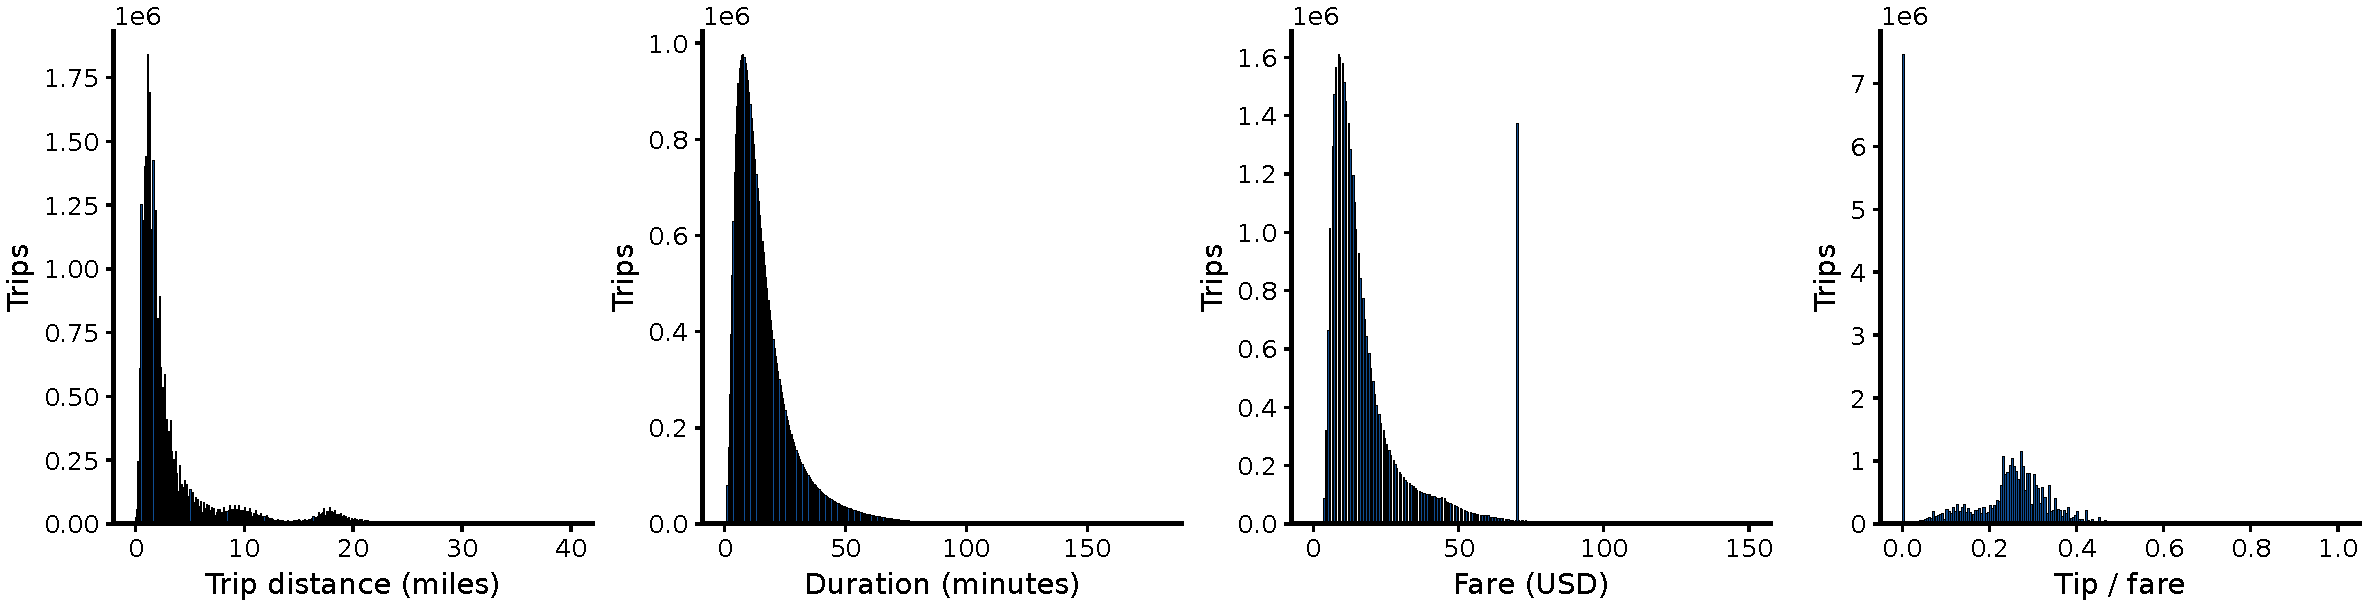
\includegraphics[width=\textwidth]{fig03_histograms}
\caption{Histograms of the cleaned rows in the twelve 2023 files. Bins are fixed in the ETL.}
\label{fig:hist}
\end{figure}

\subsection{Time and borough}
Of the cleaned pickups with a 2023 timestamp, 34,893,926 fall in the hour-and-borough recount. Manhattan accounts for 31,341,107 of them (89.8\%). Queens is next, with 3,415,423 (9.79\%). Brooklyn has 122,590 (0.35\%), the Bronx 10,401, Staten Island 217, Newark Airport 394, and 3,794 rows have no borough name in the lookup.

Figure~\ref{fig:heat} is the same recount by hour and day of week. The busiest cell is Thursday at 18:00 (405,828 trips). Wednesday at 18:00 is next, with 403,169 trips, 0.7\% below that cell. Tuesday at 18:00 has 384,280. The pattern is a weekday evening peak. Weekdays hold 72.9\% of these pickups.

\begin{figure}[ht]
\centering
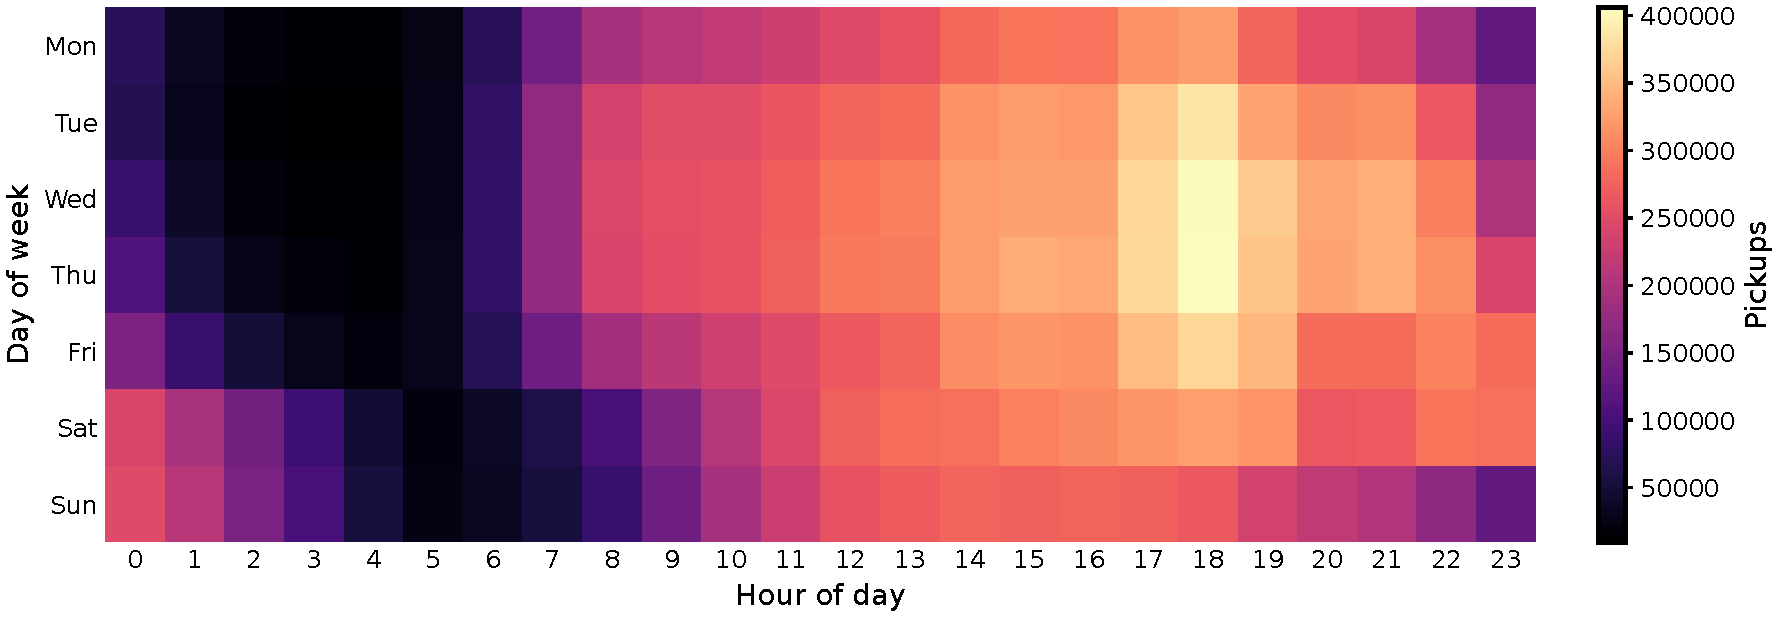
\includegraphics[width=\textwidth]{fig04_hour_dow}
\caption{Cleaned 2023 pickups by hour and weekday. The busiest cell is Thursday at 18:00.}
\label{fig:heat}
\end{figure}

Figure~\ref{fig:month} shows the monthly series and the borough totals by hour. September has 2,551,411 cleaned pickups and May has 3,215,412, which is 26.0\% higher. The year does not contain a break on the scale of a collapse. The right panel is on a logarithmic axis so Queens remains visible next to Manhattan.

\begin{figure}[ht]
\centering
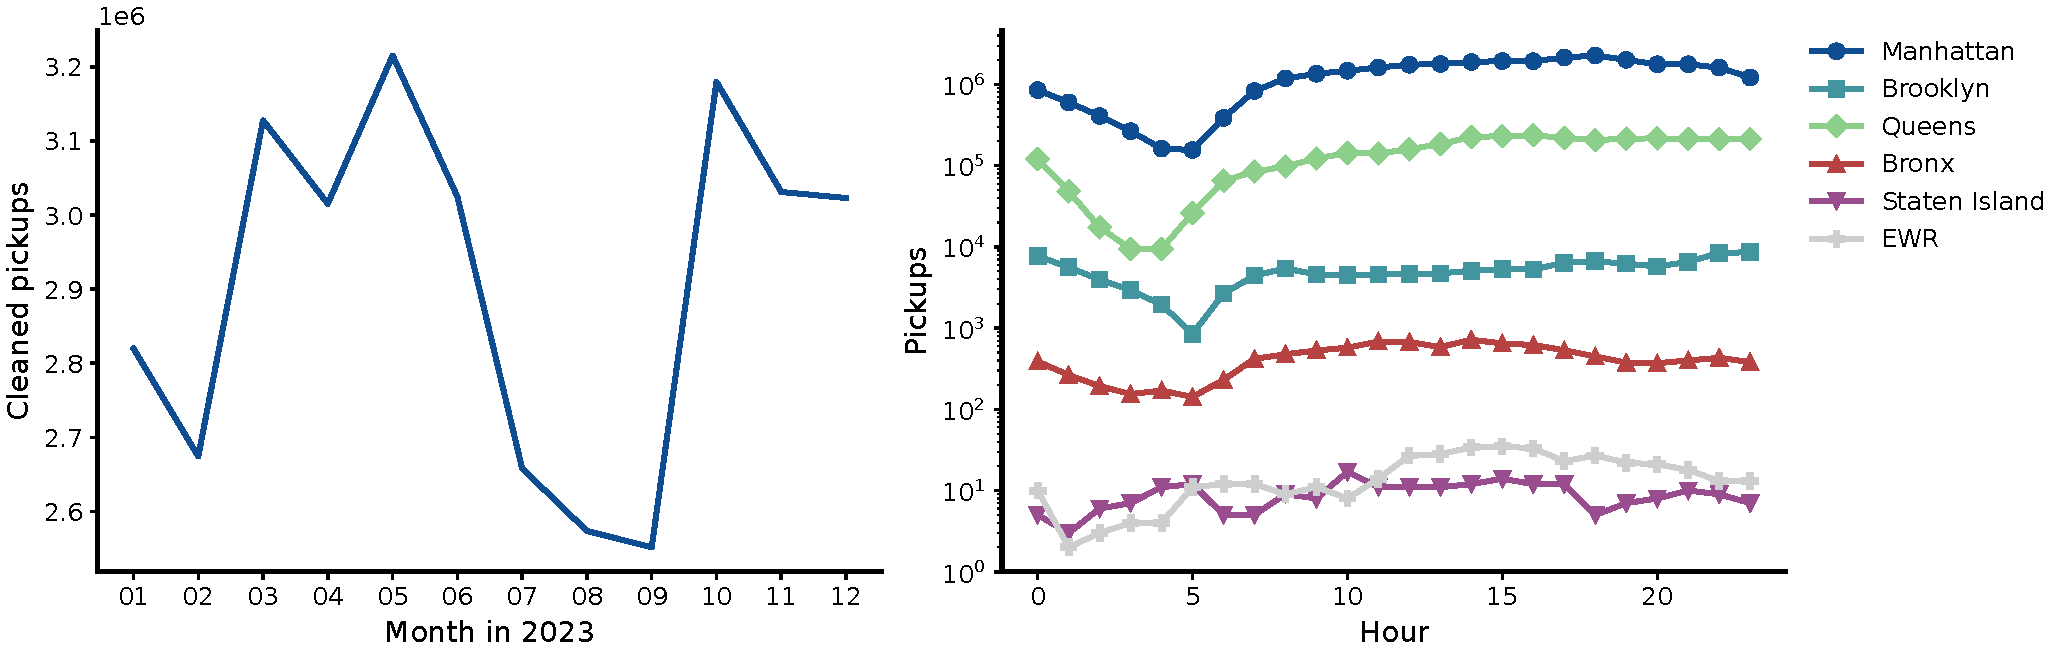
\includegraphics[width=\textwidth]{fig05_monthly_borough}
\caption{Left: cleaned pickups by month in 2023. Right: the same year by hour and borough, on a logarithmic axis.}
\label{fig:month}
\end{figure}

Two counts set the base rate for the clustering. Manhattan holds 89.8\% of dated pickups and Queens holds 9.79\%. Weekdays hold 72.9\%, and the busiest cell is Thursday at 18:00. Section~\ref{sec:clusters} shows that a two-group fit on these features isolates the Queens tail and leaves the clock mixed. The same section then keeps $k = 4$, which also splits weekday morning from weekday afternoon. That Queens tail is narrower than the borough: the \$70 spike above and the cluster in Section~\ref{sec:clusters} are both a single airport, not the 3.4 million pickups that start in Queens.

\section{Parallel design and experimental setup}
\label{sec:method}

\subsection{ETL}
Figure~\ref{fig:pipe} is the ETL. Figure~\ref{fig:tasks} names the timed workloads. The ETL and the k-means kernel are the two we use. FP-Growth is the third curve in Figure~\ref{fig:speedup}, and Section~\ref{sec:fpgrowth} says why it is not a result.

\begin{figure}[ht]
\centering
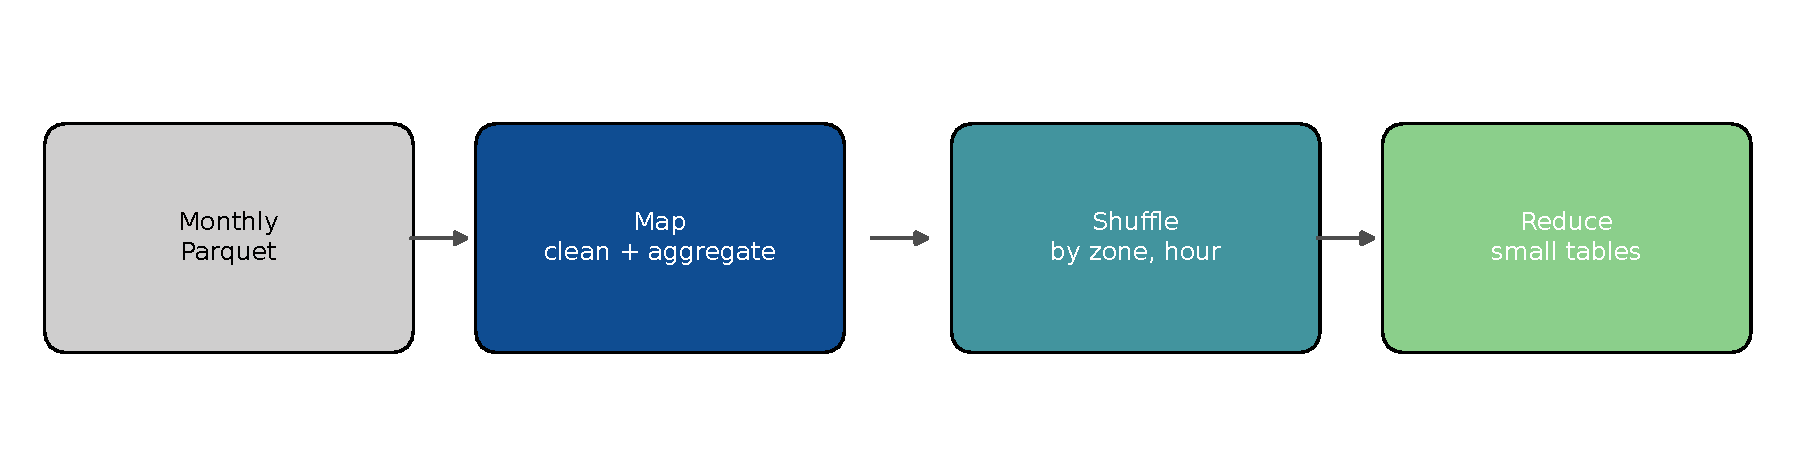
\includegraphics[width=\textwidth]{fig02_pipeline}
\caption{ETL as map, shuffle, and reduce. Each worker returns zone aggregates, not trips.}
\label{fig:pipe}
\end{figure}

\begin{figure}[ht]
\centering
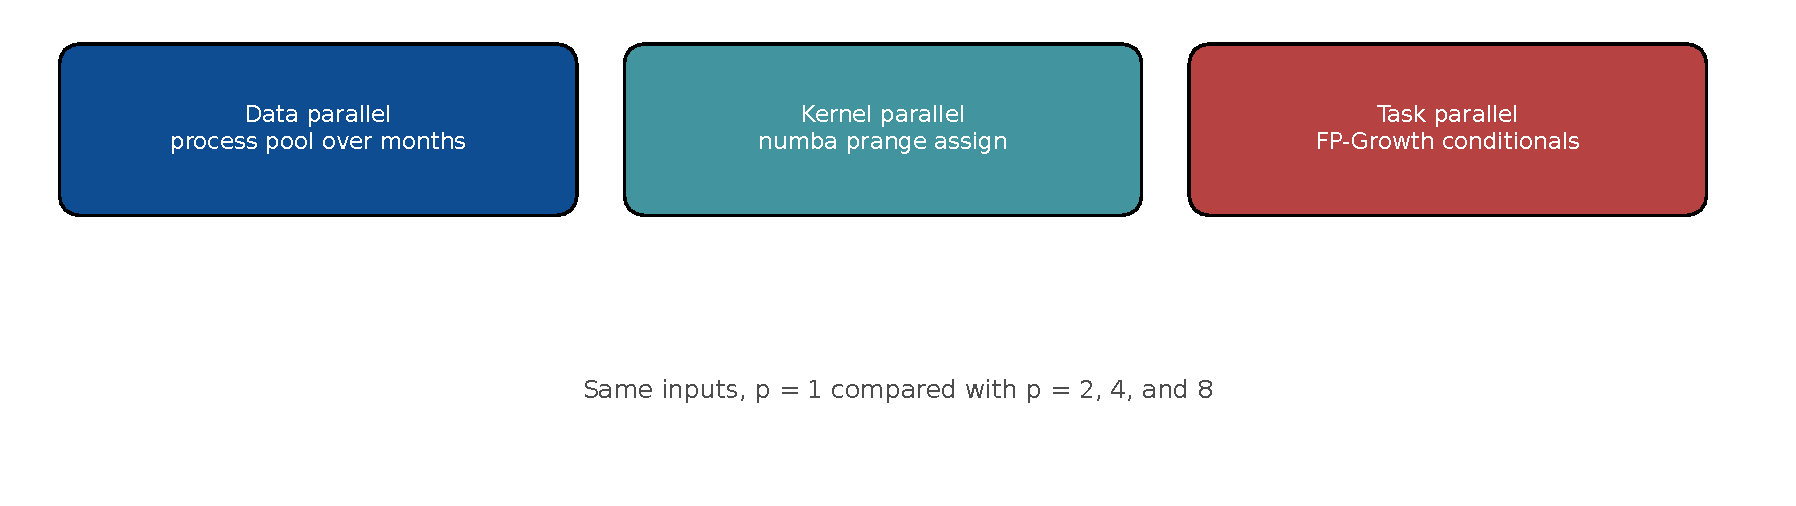
\includegraphics[width=\textwidth]{fig06_tasks}
\caption{The timed workloads. They do not share a scheduler. Each has its own $p$. The reported analysis uses the ETL and k-means.}
\label{fig:tasks}
\end{figure}

The ETL comparison is three settings of the same twelve files. The process pool varies $p$ at chunk size 1. The thread pool is run at $p = 4$. The chunk-size runs use the process pool at $p = 4$ with chunk size 4 and chunk size 12. A pure-Python loop of 400{,}000 tuples, with no NumPy, is timed separately so the GIL claim is not only a property of pandas.

\subsection{k-means}
Lloyd's algorithm alternates assignment and centroid update~\cite{lloyd1982}. Initial centres use k-means++ on a 20{,}000-row draw~\cite{arthur2007}. The assignment is a parallel \texttt{for} over blocks of rows: each point reads every centre and writes one label~\cite{lam2015}. The published labels reduce centroids in row order, so the labels do not depend on the thread count. The timed kernel reduces with a per-thread accumulator, which avoids one shared write. On a 600-point synthetic set the row-order reduction matches a NumPy implementation exactly, and the thread-local reduction stays at an adjusted Rand index of at least 0.98 against that reference.

The timing matrix uses $n = 2{,}600{,}000$ points, $k = 24$, 30 iterations, and eight standardised features. That $k$ is a compute load. The grouping in Section~\ref{sec:clusters} uses a different feature set, $k = 4$, and 200{,}000 trips from 2023.

\subsection{FP-Growth, as a limit}
FP-Growth inserts each transaction into a prefix tree and then grows a conditional tree for each frequent item~\cite{han2000}. The conditional trees do not depend on each other, so they can be separate tasks. The prefix tree is built in the parent before the pool starts. On the timed input that build is most of the wall time. The input is 1{,}200{,}000 transactions at minimum support 0.02. On 1{,}500 random transactions the miner matches \texttt{mlxtend}, and the parallel miner matches the serial miner. We stop there. Section~\ref{sec:fpgrowth} reports the wall times and does not report rules.

\subsection{Host and protocol}
The host reports an Intel Xeon at 2400 MHz, 4 logical CPUs, 4 physical CPUs, and 15.6 GiB of RAM. The model string is the hypervisor name, not a retail SKU. We pin the process to the first $\min(p, 4)$ CPUs. Numba reads the CPU count when it is imported, so the thread pool is created with 8 threads before the pin. \texttt{set\_num\_threads}$(p)$ then selects $p$ of those threads. The $p = 8$ k-means point is eight threads on four pinned cores.

Every timed configuration has one discarded warmup and then repeated measured runs. The main curves use five measured runs. Chunk-size, block-size, single-month, and weak-scaling runs use three. We store every measured run in \texttt{results/runs.csv} and plot the median. Error bars on the speedup figure span the first and third quartiles of wall time, converted with the same $T_1$. We do not drop the page cache. The warmup is there so that the measured runs share a warm cache.

\section{Results}
\label{sec:results}

Every wall time below is a median of the measured repeats in \texttt{results/runs.csv}. The main curves use five repeats after one discarded warmup. Chunk size, block size, the single-month run, and the weak-scaling runs use three. Quartile bands on Figure~\ref{fig:speedup} use the first and third quartiles of wall time and the same $T_1$. The page cache was not dropped.

\subsection{Trip groups}
\label{sec:clusters}

The grouping run is separate from the timing kernel. It draws 25{,}000 cleaned rows from each of the twelve 2023 files, keeps the 299{,}970 rows with a zone centroid, and fits 200{,}000 of those rows. The six features are the zone centroid's easting and northing, $\sin(2\pi h/24)$ and $\cos(2\pi h/24)$ for the pickup hour $h$, a weekend indicator, and $\log(1 + \text{distance})$. Each column is standardised to zero mean and unit variance. Easting and northing are the TLC shapefile's State Plane coordinates (NAD83, New York Long Island, US survey feet). A Euclidean distance in degrees of longitude and latitude would stretch the east-west axis, so the projected coordinates are the ones in the file.

Labels use the row-order centroid update, for 30 iterations, so they do not depend on the thread count. Silhouette is computed earlier, on 8{,}000 of the fitted rows, after 20 iterations. Table~\ref{tab:sil} is that curve. The maximum is $k = 2$ at 0.550. The score falls to 0.266 at $k = 3$ and is 0.312 at $k = 4$ and 0.322 at $k = 5$.

\begin{table}[ht]
\centering
\caption{Silhouette on 8{,}000 of the 200{,}000 fitted rows. Euclidean distance in the six standardised features. The maximum is $k = 2$. The groups in Table~\ref{tab:clusters} use $k = 4$.}
\label{tab:sil}
\begin{tabular}{cccccccc}
\toprule
$k$ & 2 & 3 & 4 & 5 & 6 & 7 & 8 \\
\midrule
Score & 0.550 & 0.266 & 0.312 & 0.322 & 0.308 & 0.263 & 0.308 \\
\bottomrule
\end{tabular}
\end{table}

The $k = 2$ fit is a length and borough split. One group has 188{,}888 rows (94.4\%), mean distance 2.76 miles, mean hour 14.3, and 95.0\% Manhattan. The other has 11{,}112 rows (5.6\%), mean distance 16.1 miles, mean hour 14.6, and 99.7\% Queens. The two mean hours differ by 0.3 hours. A higher silhouette here is one airport against the city, not a split by time of day.

We report $k = 4$, not the silhouette maximum. The $k = 5$ score is 0.010 higher than $k = 4$, and the fifth group is a night cluster that mixes weekdays and weekends. The four groups in Table~\ref{tab:clusters} each have one reading. Cluster 3 is weekday morning and midday (mean hour 10.5, weekend share 0, midday share 64.7\%). Cluster 0 is weekday afternoon and evening (mean hour 17.7, weekend share 0, afternoon plus evening 67.8\%). Cluster 2 is the weekend (weekend share 100\%, mean hour 13.3). Cluster 1 is the JFK group (99.7\% Queens, mean distance 16.1 miles, mean duration 42.0 minutes, mean fare \$63.69). Mean distance in the three Manhattan groups stays between 2.68 and 2.84 miles.

\begin{table}[ht]
\centering
\caption{k-means profiles on 200{,}000 trips from 2023, $k = 4$. Cluster ids are the labels from the fit. The order of columns follows the reading in the text, not the id order.}
\label{tab:clusters}
\small
\setlength{\tabcolsep}{5pt}
\begin{tabular}{lrrrr}
\toprule
 & C3 & C0 & C2 & C1 \\
\midrule
Rows & 58,084 & 79,950 & 50,874 & 11,092 \\
Share & 29.0\% & 40.0\% & 25.4\% & 5.5\% \\
Mean distance (miles) & 2.81 & 2.68 & 2.84 & 16.10 \\
Mean duration (minutes) & 15.8 & 14.6 & 13.9 & 42.0 \\
Mean fare (USD) & 17.80 & 16.67 & 16.82 & 63.69 \\
Mean pickup hour & 10.5 & 17.7 & 13.3 & 14.6 \\
Weekend share & 0\% & 0\% & 100\% & 28.7\% \\
Manhattan share & 94.7\% & 94.9\% & 95.4\% & 0\% \\
Queens share & 4.9\% & 4.8\% & 4.0\% & 99.7\% \\
\bottomrule
\end{tabular}
\end{table}

Cluster 1 is one airport, not the borough. Zone 132, JFK Airport, accounts for 10,903 of its 11,092 rows, or 98.3\%. The other 189 rows are spread over 41 zones: 161 rows in 24 other Queens zones, and 28 rows in 17 Brooklyn zones. LaGuardia, zone 138, is not in this group. Its 7,243 sampled pickups fall in clusters 0, 2, and 3. The remaining Queens pickups are not lost. Clusters 0, 2, and 3 draw 4.8\%, 4.0\%, and 4.9\% of their rows from Queens, and their mean distance stays between 2.68 and 2.84 miles. Only the JFK trips are long and expensive enough to stand apart. That reading matches the fare spike in Section~\ref{sec:eda}.

Weekend share is 0 or 1 in the three Manhattan groups because the weekend indicator is one of the six inputs. That cluster is the coordinate being used, not a pattern found in spite of it. The morning and afternoon split is not a pre-cut label: the clock enters only as $\sin$ and $\cos$ of the hour. The airport group agrees in both geography and distance. Its zone centroid sits far from Manhattan, and its mean distance is 16.1 miles against 2.7--2.8 miles in the other three groups. We did not drop either feature, so this fit does not say which of the two is sufficient. The four groups are the $k = 4$ cut of this feature set. $k = 2$ remains the silhouette maximum, and it is the same airport tail before the clock is split.

\begin{figure}[ht]
\centering
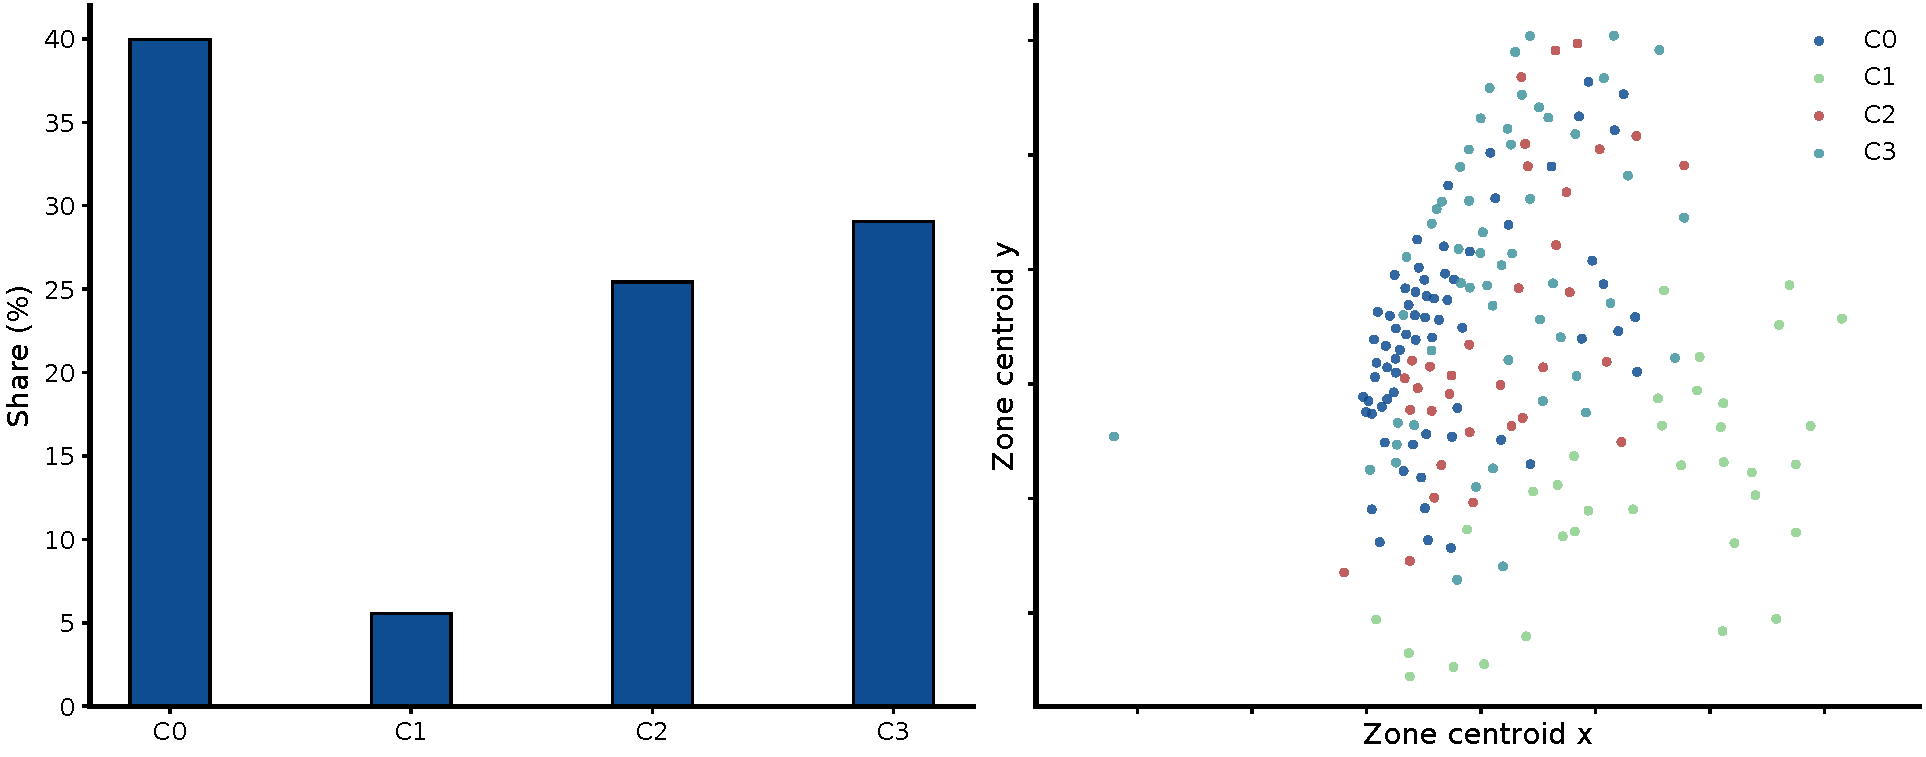
\includegraphics[width=\textwidth]{fig07_clusters}
\caption{Left: share of the 200{,}000 fitted rows. Right: zone centroids coloured by the majority cluster among sampled pickups in that zone. The three Manhattan groups share the same zones, so the majority colour on Manhattan is cluster 0, the larger weekday group. Zone 132, JFK Airport, takes cluster 1. A few neighbouring Queens zones share that colour on a small sample. Cluster 2, the weekend, has no zone of its own.}
\label{fig:clusters}
\end{figure}

\FloatBarrier
\subsection{ETL: processes, threads, and chunk size}
\label{sec:speedup}

Figure~\ref{fig:speedup} plots $S(p)$ for the ETL, the k-means kernel, and FP-Growth. The dashed line is $S(p) = p$. Table~\ref{tab:t1} is the process-pool ETL on the twelve files, chunk size 1.

\begin{figure}[ht]
\centering
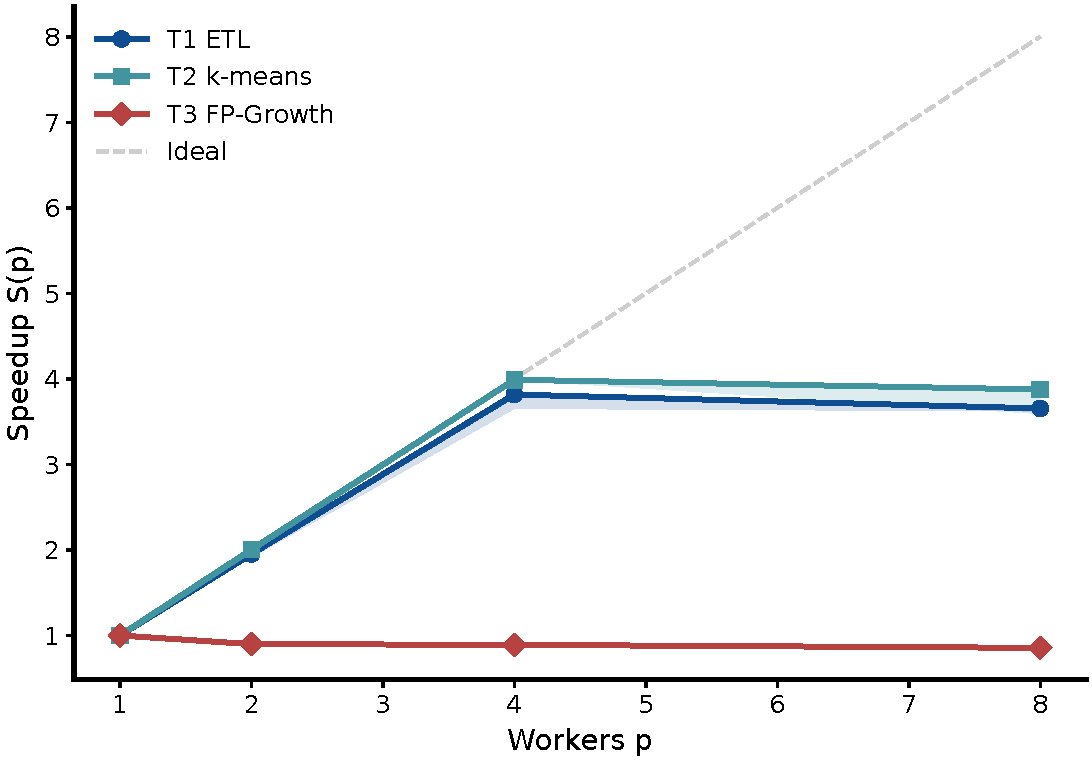
\includegraphics[width=0.86\textwidth]{fig09_speedup}
\caption{Warm-cache speedup. Bands convert the first and third quartiles of wall time with the same $T_1$. The dashed line is ideal speedup. $p = 8$ is eight workers on four cores.}
\label{fig:speedup}
\end{figure}

\begin{table}[ht]
\centering
\caption{ETL, twelve files of 2023, process pool, chunk size 1. Five repeats.}
\label{tab:t1}
\begin{tabular}{rrrr}
\toprule
$p$ & Median (s) & $S(p)$ & $E(p)$ \\
\midrule
1 & 52.135 & 1.00 & 1.000 \\
2 & 26.717 & 1.95 & 0.976 \\
4 & 13.658 & 3.82 & 0.954 \\
8 & 14.266 & 3.65 & 0.457 \\
\bottomrule
\end{tabular}
\end{table}

The process pool is close to linear through four workers: $S(2) = 1.95$ and $S(4) = 3.82$. Median system CPU moves from 25\% to 50\% to 100\%. At $p = 8$ the median rises from 13.658 s to 14.266 s and CPU stays at 100\%. There is no fifth core for the extra processes.

The same twelve files on a thread pool at $p = 4$ take 27.423 s, with median CPU 42.3\%. Relative to the one-process median of 52.135 s, that is $S = 1.90$. The process pool at the same $p$ takes 13.658 s and uses 100\% CPU. Pandas and Arrow release the GIL for part of the read and the numeric work, which is why four threads still beat one process. The cleaning rules keep the rest on one interpreter, which is why four processes beat four threads. The ETL uses processes for that reason.

A separate pure-Python loop, 400{,}000 tuples and no NumPy, checks the same mechanism on code that cannot release the GIL. Threads take 0.0179 s at $p = 1$ and 0.0195 s at $p = 4$. Processes take 0.292 s and 0.201 s. The pool costs more than the loop, so processes are slower in absolute time. The GIL evidence in Figure~\ref{fig:gil} is the flat thread bar. The pool decision uses the 27.423 s and 13.658 s above, not this figure.

\begin{figure}[ht]
\centering
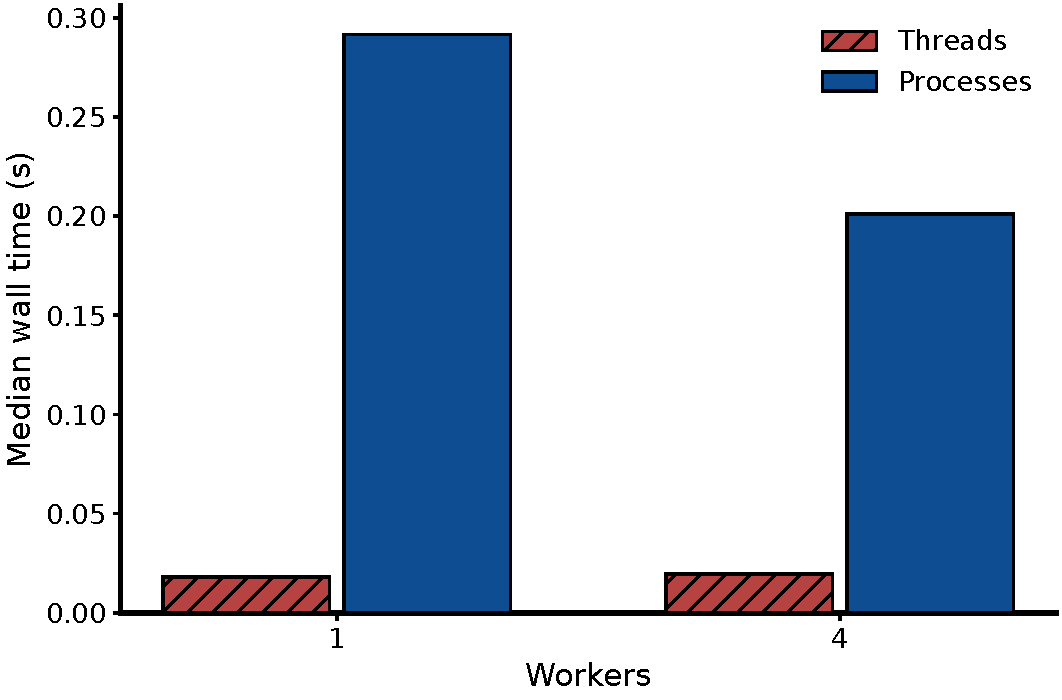
\includegraphics[width=0.72\textwidth]{fig12_gil}
\caption{Pure-Python row loop, 400{,}000 tuples. Threads stay near 0.02 s. Process startup dominates the same loop.}
\label{fig:gil}
\end{figure}

Chunk size is the number of files one worker receives in a batch. At $p = 4$, chunk size 1 takes 13.658 s. Chunk size 4 takes 17.038 s, and median CPU falls to 76.2\%. Chunk size 12 takes 49.668 s, and median CPU is 25.3\%. Twelve files in one chunk leave a single worker holding the year. The other three processes have nothing to run. A single file, January 2023, takes 4.579 s at $p = 1$ and 4.195 s at $p = 4$ ($S = 1.09$). One file cannot fill four workers, because the file is the unit of work.

\FloatBarrier
\subsection{Where the ETL time goes}
\label{sec:phases}

Figure~\ref{fig:phases} stacks three timers from the worker processes and draws wall time on top. The timers are summed across files and then divided by $p$. At $p = 1$ the medians are 1.600 s to read, 19.916 s to clean, and 26.527 s to aggregate. The stack is 48.0 s against a wall of 52.135 s. The gap is pool and interpreter time outside those three timers. Read is a small slice once the cache is warm.

\begin{figure}[ht]
\centering
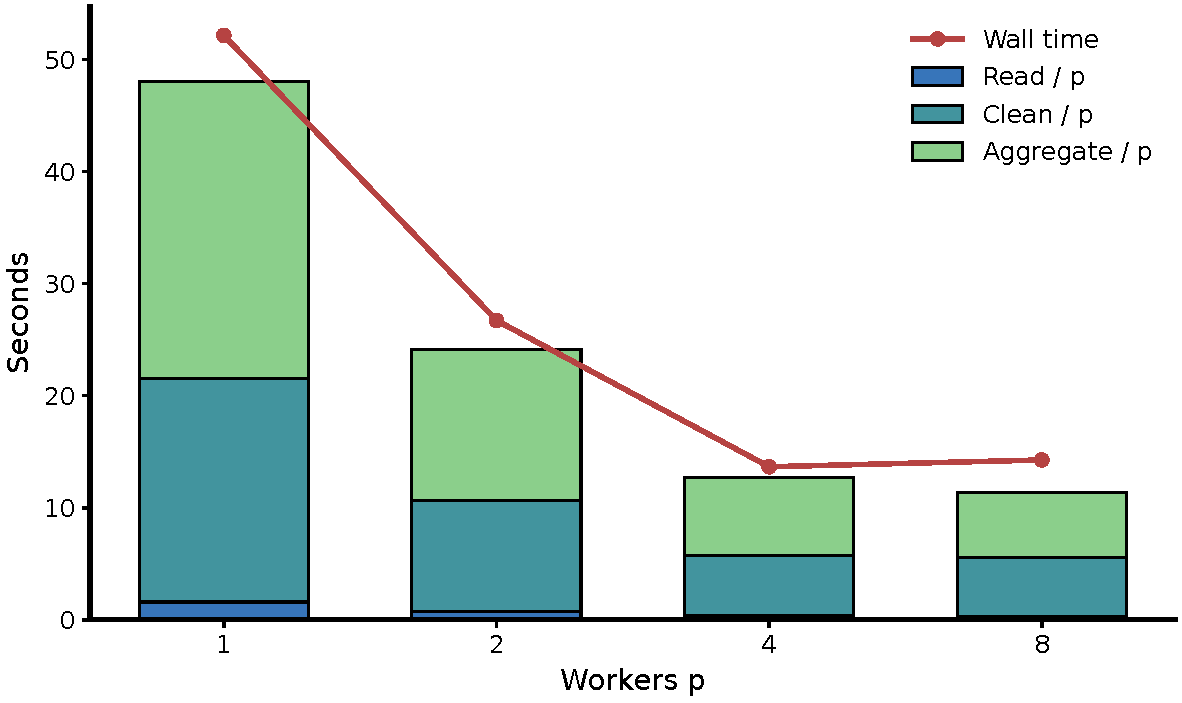
\includegraphics[width=0.86\textwidth]{fig10_phases}
\caption{ETL phases for the twelve files of 2023. Each bar is the summed phase CPU divided by $p$. The line is wall time. Through $p = 4$ the stack and the line fall together. At $p = 8$ the wall stops falling.}
\label{fig:phases}
\end{figure}

At $p = 4$ the summed clean and aggregate times stay near the serial sums (21.395 s and 27.954 s) while the wall falls to 13.658 s. At $p = 8$ those sums rise to 42.167 s and 46.218 s. Dividing by 8 makes the stack in the figure shorter than at $p = 4$, but the raw CPU grew, and the wall rose to 14.266 s. The extra processes wait on the same four cores. The bytes that cross the process boundary are the zone aggregates, not the trips. That reduce is small next to the clean and the aggregate, which is why $S(4)$ can reach 3.82. It does not remove the limit at four cores.

\FloatBarrier
\subsection{k-means speedup}
\label{sec:kmeans}

Table~\ref{tab:t2} is the timing kernel: 2{,}600{,}000 points, $k = 24$, 30 iterations, block 8{,}192, thread-local centroid update. This $k$ and these eight features are a compute load. They are not the $k = 4$ fit in Section~\ref{sec:clusters}.

\begin{table}[ht]
\centering
\caption{k-means, 2{,}600{,}000 points, $k = 24$, 30 iterations, block 8{,}192, thread-local update. Five repeats.}
\label{tab:t2}
\begin{tabular}{rrrr}
\toprule
$p$ & Median (s) & $S(p)$ & $E(p)$ \\
\midrule
1 & 6.428 & 1.00 & 1.000 \\
2 & 3.208 & 2.00 & 1.002 \\
4 & 1.611 & 3.99 & 0.997 \\
8 & 1.659 & 3.88 & 0.484 \\
\bottomrule
\end{tabular}
\end{table}

$S(2) = 2.00$ and $S(4) = 3.99$. The $p = 2$ point is slightly above 2. Replacing each median by the opposite quartile puts that speedup between 1.96 and 2.03, so the excess sits inside the repeat spread. At $p = 8$ the median rises from 1.611 s to 1.659 s. Eight threads are running on four pinned cores, and the wall stops falling.

Weak scaling keeps about 650{,}000 points per thread. The medians are 1.407 s at $p = 1$ (650{,}000 points), 1.575 s at $p = 2$ (1{,}300{,}000 points), and 1.624 s at $p = 4$ (2{,}600{,}000 points). Time rises 12\% and then 15\% while the row count quadruples. Ideal weak scaling would hold the time fixed. The 15\% rise is the departure from that line on this host.

Figure~\ref{fig:blocksize} varies the block at $p = 4$ on the same 2{,}600{,}000 points. Table~\ref{tab:block} lists the medians. The fastest block is 64 rows (1.594 s). The slowest is 262{,}144 rows (1.912 s). The range is 0.32 s. Between 1{,}024 and 65{,}536 rows the median stays inside 1.620--1.661 s, next to the 8{,}192-row point used in Table~\ref{tab:t2} (1.611 s). We do not read a preferred block size from that range. Worker count moves the median from 6.428 s to 1.611 s. Block size does not.

\begin{figure}[ht]
\centering
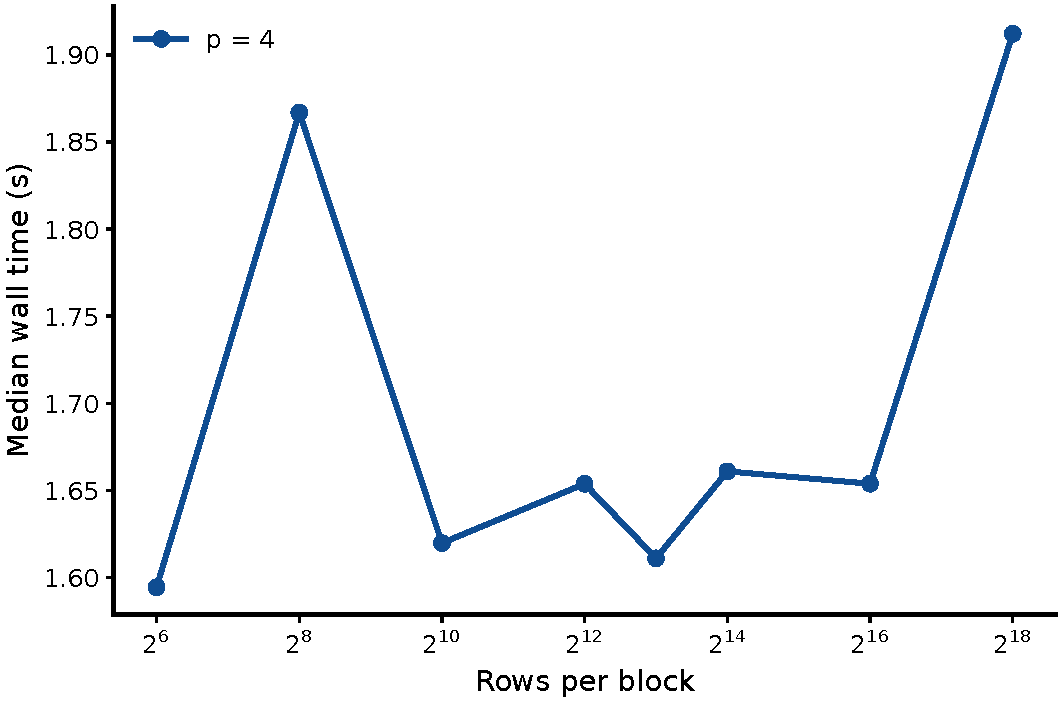
\includegraphics[width=0.78\textwidth]{fig11_blocksize}
\caption{k-means wall time against rows per block, $p = 4$, three repeats. The vertical range is 1.59--1.91 s.}
\label{fig:blocksize}
\end{figure}

\begin{table}[ht]
\centering
\caption{Block-size medians at $p = 4$. Three repeats, except 8{,}192 rows, which is the five-repeat entry from Table~\ref{tab:t2}.}
\label{tab:block}
\begin{tabular}{rr}
\toprule
Rows per block & Median (s) \\
\midrule
64 & 1.594 \\
256 & 1.867 \\
1,024 & 1.620 \\
4,096 & 1.654 \\
8,192 & 1.611 \\
16,384 & 1.661 \\
65,536 & 1.654 \\
262,144 & 1.912 \\
\bottomrule
\end{tabular}
\end{table}

\FloatBarrier
\subsection{A split that does not speed up}
\label{sec:fpgrowth}

FP-Growth was timed because the assignment lists association rules. We do not use the itemsets as a finding. On the inputs we tried, the frequent combinations restated long trips and payment type, and they did not add a travel pattern beyond Table~\ref{tab:clusters}. The timing result is still useful as a limit on this kind of parallelism.

The tree is built in the parent before the process pool starts. The pool then grows one conditional tree per frequent item~\cite{han2000}. Those tasks do not depend on each other. On 1{,}200{,}000 transactions at minimum support 0.02, the parent build dominates the measured time. Table~\ref{tab:t3} is the wall time. It rises from 1.497 s at one worker to 1.666 s, 1.681 s, and 1.750 s. $S(4) = 0.89$ and $S(8) = 0.86$. Median system CPU stays between 25.3\% and 25.6\% at every $p$. Extra processes do not occupy extra cores for most of that second and a half.

\begin{table}[ht]
\centering
\caption{FP-Growth, 1{,}200{,}000 transactions, minimum support 0.02. Five repeats.}
\label{tab:t3}
\begin{tabular}{rrrr}
\toprule
$p$ & Median (s) & $S(p)$ & $E(p)$ \\
\midrule
1 & 1.497 & 1.00 & 1.000 \\
2 & 1.666 & 0.90 & 0.449 \\
4 & 1.681 & 0.89 & 0.223 \\
8 & 1.750 & 0.86 & 0.107 \\
\bottomrule
\end{tabular}
\end{table}


\FloatBarrier
\section{Discussion}
\label{sec:discuss}

The curves in Figure~\ref{fig:speedup} do not support one speedup for the project. At $p = 4$ the ETL reaches 3.82 and k-means reaches 3.99. Both already sit on a fully busy machine at $p = 4$ (system CPU at 100\% for the process pool, and for the k-means kernel). Moving to $p = 8$ makes each of them slower: 13.658 s to 14.266 s for the ETL, and 1.611 s to 1.659 s for k-means. FP-Growth goes the other way. $S(4) = 0.89$, and system CPU stays near 25\%. The code splits into a serial tree build and a process pool, and on this input the pool does not fill the host.

The pool comparison is the ETL one. At $p = 4$ the thread pool takes 27.423 s and the process pool takes 13.658 s. Threads still beat one process (52.135 s), so part of the ETL releases the GIL. The pure-Python loop does not: threads take 0.0179 s at $p = 1$ and 0.0195 s at $p = 4$. Chunk size is the other ETL control. Chunk size 12 at $p = 4$ takes 49.668 s with CPU at 25.3\%, against 13.658 s at chunk size 1. The serial part, in that setting, is the decision to hand every file to one worker.

We did not run Spark. The twelve files finish in under a minute once four processes are used, and the aggregates fit in memory~\cite{zaharia2012}. A larger table would raise that question again. It is unmeasured here.

The study has several limits. Timings share a warm page cache, and the CPU is a virtual Xeon with four cores. k-means assumes spherical clusters in the standardised features. Silhouette uses 8{,}000 of the 200{,}000 fitted rows, and the reported labels are a 30-iteration refit rather than the 20-iteration pass that produced the silhouette. Weekend is an input, so a weekend share of 0 or 1 is that coordinate. The zone centroid is the mean of the shapefile vertices, not a count of pickups inside the polygon. Yellow trips are not the full for-hire market. Duplicate removal does not cross the 1{,}000{,}000-row batch boundary. In 2023 that boundary hides 2 within-batch duplicates, so a global pass would not move Table~\ref{tab:rules}.

\section{Conclusion}
\label{sec:conclusion}

In the twelve yellow-taxi files of 2023, 34,893,980 of 38,310,226 rows survive the seven cleaning rules. Of the dated pickups, 89.8\% start in Manhattan and 9.79\% start in Queens. Weekdays hold 72.9\%, and the busiest cell is Thursday at 18:00 (405,828 trips). May is 26.0\% above September. There is no within-year break in the monthly series.

k-means on zone location, time of day, weekend, and log distance has its silhouette maximum at $k = 2$ (0.550). That cut is the JFK tail against the rest, and the two mean hours differ by 0.3 hours. We report $k = 4$ (silhouette 0.312). The four groups are weekday morning, weekday afternoon and evening, weekend, and a JFK group at 16.1 miles and \$63.69. The weekend group uses an input indicator. The morning and afternoon groups are a split of the hour. The JFK group is the same tail that $k = 2$ isolates, kept as its own group once $k$ is large enough to also split the clock.

On this 4-core host the process-pool ETL moves from 52.135 s at $p = 1$ to 13.658 s at $p = 4$ ($S = 3.82$) and slows to 14.266 s at $p = 8$. A thread pool at $p = 4$ takes 27.423 s. Chunk size 12 at $p = 4$ takes 49.668 s because one worker receives every file. The k-means kernel moves from 6.428 s to 1.611 s ($S = 3.99$) and slows at $p = 8$. FP-Growth does not speed up at any $p > 1$ ($S(4) = 0.89$), and we do not report its itemsets. The practical rule from these measurements is to put the Python cleaning in a process pool, to keep the chunk size at one file, and to treat a serial tree build as work that more processes will not shrink.

\section*{Contribution statement}
\label{sec:contrib}
All four members contributed equally (25\% each).

\begin{quote}
WANG Shen (60216681): 25\%. Data acquisition, the seven cleaning rules, the process-pool ETL, and integration of the full manuscript. Sections 3 and 4, and the ETL design in Section 5.

LIU Wanyang (60915652): 25\%. Serial and \texttt{prange} k-means, the FP-Growth timing kernel, and the equivalence tests. Section 5.

WANG Yuwei (60875477): 25\%. Exploratory figures and the cluster profiles. Sections 4 and 6.1.

YU Xiyan (61076721): 25\%. The scaling matrix, the speedup analysis, and the slides. Sections 1, 2, 6.2 to 6.5, 7, and 8.
\end{quote}

\begingroup
\raggedright
\bibliography{refs}
\endgroup

\end{document}
